\chapterimage{./Pictures/cover-inheritance} % Chapter heading image
\chapter{TP9+TP10 : Héritage multiple et modélisation}
\textit{Ce TP nous permet de manipuler de manière concrète des mécanismes caractéristiques de la programmation orientée objet tels que la notion de classe, d’objet, d’héritage ainsi que l’héritage multiple, qui est propre au langage de programmation C++.
Pour voir ces différentes notions nous allons créer un jeu simple.}

Afin de structurer un projet et avoir un code aussi clair que possible en c++, il est conseillé de séparer son
code en deux types de fichiers : les fichiers d’en-têtes \texttt{header (.h)} servant à définir les classes et
donnant les différents prototype de méthodes, et les fichiers avec l’extension \texttt{.cpp}, que l’on devra compiler et qui contiennent tout le code des méthodes. On créé également un fichier main.cpp , que l’on doit compiler et qui contiendra la logique du jeu.
Les fichiers \texttt{.h} sont inclus dans les fichiers \texttt{.cpp} correspondants ainsi que dans le main afin que l’on puisse avoir accès à la déclaration des classes et leurs prototypes de méthodes.
Les fichiers .cpp sont compilés ensemble avec le compilateur g++ en un seul fichier exécutable.

Le jeu est un affrontement entre des peronnages, pouvant être de différents types : Guerrier, Mage ou Mage-Guerrier.
Afin d'organiser ses idées et de bien commencer une programmation orientée object, on propose de modéliser les classes à l'aide du diagramme de classe suivant :

\begin{figure}[H]
\centering
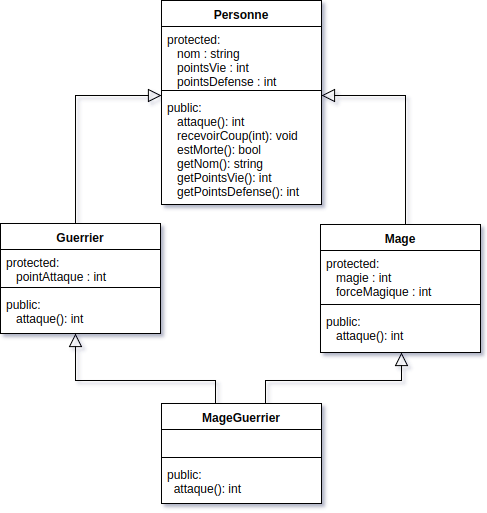
\includegraphics[width=400pt]{./cpp/Pictures/tp9+10-inheritance}
\caption{Diagramme de classe}
\label{Diagramme de classe}
\end{figure}

En premier nous allons définir la classe \texttt{Personne}, qui permet de définir les attributs communs à tous les combattants : le nom, de type \mintinline{cpp}{string} (chaîne de caractère), les points de vie et les points de défense, de type \mintinline{cpp}{int}. Ces attributs auront le spécificateur d’accès \mintinline{cpp}{protected}. Ce spécificateur précise que de sattributs sont accessibles au sein de la classe ainsi que ses classes filles.
Nous allons donc créer des accesseurs en lecture afin de pouvoir lire les attributs des instances de la classe \texttt{Personne} dans le main si nécessaire avec des fonctions méthodes tels que :

\inputminted[linenos,firstline=33, lastline=35]{cpp}{../sources/cpp/TP9-10/Personne.cpp}

Afin d'initialiser correctement les membres de l'objet, on peut créer un constructeur et lui passer les valeurs que nous voulons attribués à l'initialisation de l'objet.

\inputminted[linenos,firstline=9, lastline=13]{cpp}{../sources/cpp/TP9-10/Personne.cpp}

On ajoute de plus la méthode \mintinline{cpp}{recevoirCoup()} afin de permettre à une personne de recevoir un coup et faire baisser ses points de vie en fonction de ses points de défense. Nous pouvons directement accéder un attribut depuis la classe en écrivant le nom de la variable, nous pouvons aussi préciser qu'il s'agit de l'attribut de l'instance actuelle avec \mintinline{cpp}{this}.

\inputminted[linenos,firstline=23, lastline=27]{cpp}{../sources/cpp/TP9-10/Personne.cpp}

On ajoute la méthode \mintinline{cpp}{attaque()} afin que chaque personne puisse attaquer. Au niveau de la classe \texttt{Personne}, cette méthode est définit comme virtuel pure et ne sera pas définit et devra donc être redéfinit dans es classes filles. La classe \texttt{Personne} n'est plus instanciable.

\inputminted[linenos,firstline=14, lastline=38]{cpp}{../sources/cpp/TP9-10/Personne.h}

Comme dit précédemment les peronnes peuvent être, de différents type dans ce jeu. Nous allons donc créé deux classes : \texttt{Guerrier} et \ texttt{Mage} héritant de la classe \texttt{Personne} (héritage simple).
Ces classes auront accès aux même attributs mais auront en plus leur propre attributs et devront redéfinir la méthode \mintinline{cpp}{attaque()} et implémenteront leur propre logique.
Ces deux classes auront aussi un constructeur pour initiliser leur propre attribut et devront appeler le constructeur de leur classe mère \texttt{Personne}.

La classe Guerrier :
\inputminted[linenos,firstline=12, lastline=23]{cpp}{../sources/cpp/TP9-10/Guerrier.h}

La classe Mage :
\inputminted[linenos,firstline=12, lastline=26]{cpp}{../sources/cpp/TP9-10/Mage.h}

Cet exercice nous propose d'hériter de deux classe, celà s'appel l'héritage multiple qui est un mécanisme de programmation orientée objet dans lequel une classe peut hériter de comportements et de fonctionnalités de plus d'une super-classe.
Ainsi nous pouvons créer un troisieme type de personnage \texttt{MageGuerrier} qui héritera à la fois de la classe \texttt{Mage} et de la classe \texttt{Guerrier}, bien entendu il héritera aussi inderectement de la classe Personne.
Le constructeur devra comme pour les classes précédentes appeler les constructeur parents, donc ici les constructeur des classes \texttt{Personne}, \texttt{Guerrier} et \texttt{Guerrier}.
Comme demander dans l'exercice on redéfinira la méthode \mintinline{cpp}{attaque()} qui devra attaquer "tantôt avec la magie, tantôt avec une attaque physique" (en tant que \texttt{Mage} ou en tant que \texttt{Guerrier}). On peut grâce à l'opérateur \mintinline{cpp}{::} appeler la méthode de notre choix, par exemple \mintinline{cpp}{Mage::attaque()} utilisera la méthode \mintinline{cpp}{attaque()} de la classe \texttt{Mage}.

La classe MageGuerrier :
\inputminted[linenos,firstline=7, lastline=21]{cpp}{../sources/cpp/TP9-10/MageGuerrier.cpp}

Afin de tester nos classe et simuler un jeu nous avons implementer un combat dans le fichier \texttt{main.cpp}.
Nous utiliserons la fonction \mintinline{cpp}{combat()} afin de simuler un combat entre deux personnes, pour cela nous devrons passer en paramètre les deux protagonistes.
Afin de pouvoir passer n'importe quel type de personnage (\texttt{Guerrier}, \texttt{Mage} et \texttt{MageGuerrier}) il sera important de préciser le type des arguments à \mintinline{cpp}{Personne *} ce qui donne \mintinline{cpp}{combat(Personne * p1, Personne *p2)}.
On applique ici le mécanisme de polymorphisme d'héritage qui permet de faire abstraction des détails des classes spécialisées d'une famille d'objet, en les masquant par une interface commune (qui est la classe de base).

Afin d'eviter les fuites mémoire à la fin de l'éxécution du programme il faut \mintinline{cpp}{delete} les objets créés.

\inputminted[linenos,firstline=43, lastline=62]{cpp}{../sources/cpp/TP9-10/main.cpp}
